\chapter{DEMONSTRATION}
    \section{Scenario}
    \subsection{Manager}
    \begin{itemize}
        \item The Manager logs in to the website using their manager credentials. Once logged in, the manager is directed to the dashboard where they can see the functions they can manage on the website. The manager can then navigate to different sections of the website, such as the front desk, room, reservation, etc.
        \item In the front desk section, the Manager can see the room being used by day, week, month and the Manager can add bookings.
        \item In the front desk section, the Manager can see the room being used and can add a booking.
        \item In the room section, the manager can add, edit, or delete a room from the website. The manager can also manage product categories, adjust pricing, and update room descriptions.
        \item In the reservation section, the manager can edit, and add meals for a room from the website. The manager can see all reservations.
        \item In the invoice section, the manager can view all invoices, total revenue, room revenue, food revenue, and transfer revenue. Additionally, the manager can search for a certain invoice.
        \item In the feedback section, the manager can see all guest reviews for the hotel.
        \item In the services section, the manager can view guests who use the airport pick-up service. Includes guest information, means of transportation used by guests, and pick-up location.
        \item In the meal section, the manager views the food that the hotel provides to serve guests. Includes dish name, type, ingredients, and price.
    \end{itemize}
    \subsection{Receptionist}
    \begin{itemize}
        \item In the front desk section, the receptionist can see the room being used and can add a booking.
        \item In the reservation section, the receptionist can edit, and add meals for a room from the website. The manager can see all reservations.
        \item In the send feedback section, the receptionist can send feedback to the manager to respond to hotel issues.
    \end{itemize}
    \subsection{Accountant}
    \begin{itemize}
        \item In the invoice section, the accountant can view all invoices, total revenue, room revenue, food revenue, and transfer revenue. Additionally, the accountant can search for a certain invoice.
    \end{itemize}
    \section{Demo}
    \subsection{Login}
    \begin{itemize}
        \item Manager, Accountant and receptionist log in to the website homepage and enter the link to access with permission:
        \begin{itemize}
            \item Manager: localhost:8080/manager
            \item Receptionist: localhost:8080/receptionist
            \item After entering the path, the system will take the actor to the login page:
            \begin{figure}[H]
                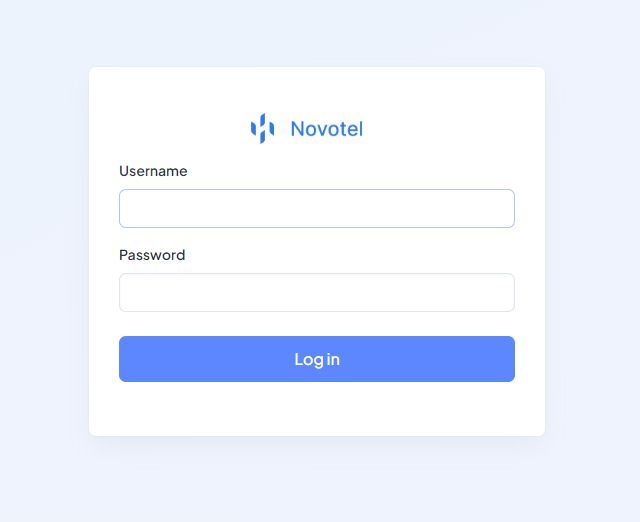
\includegraphics[width=1\linewidth]{img/login.png}
                \label{fig:Login}
            \end{figure}
        \end{itemize}
    \end{itemize}
    \subsection{Check for available rooms}
    \begin{itemize}
        \item Guest, Receptionist, and Manager access the home page and fill in the time they will check in, check out, and the number of people who will rent the room.
        \begin{figure}[H]
            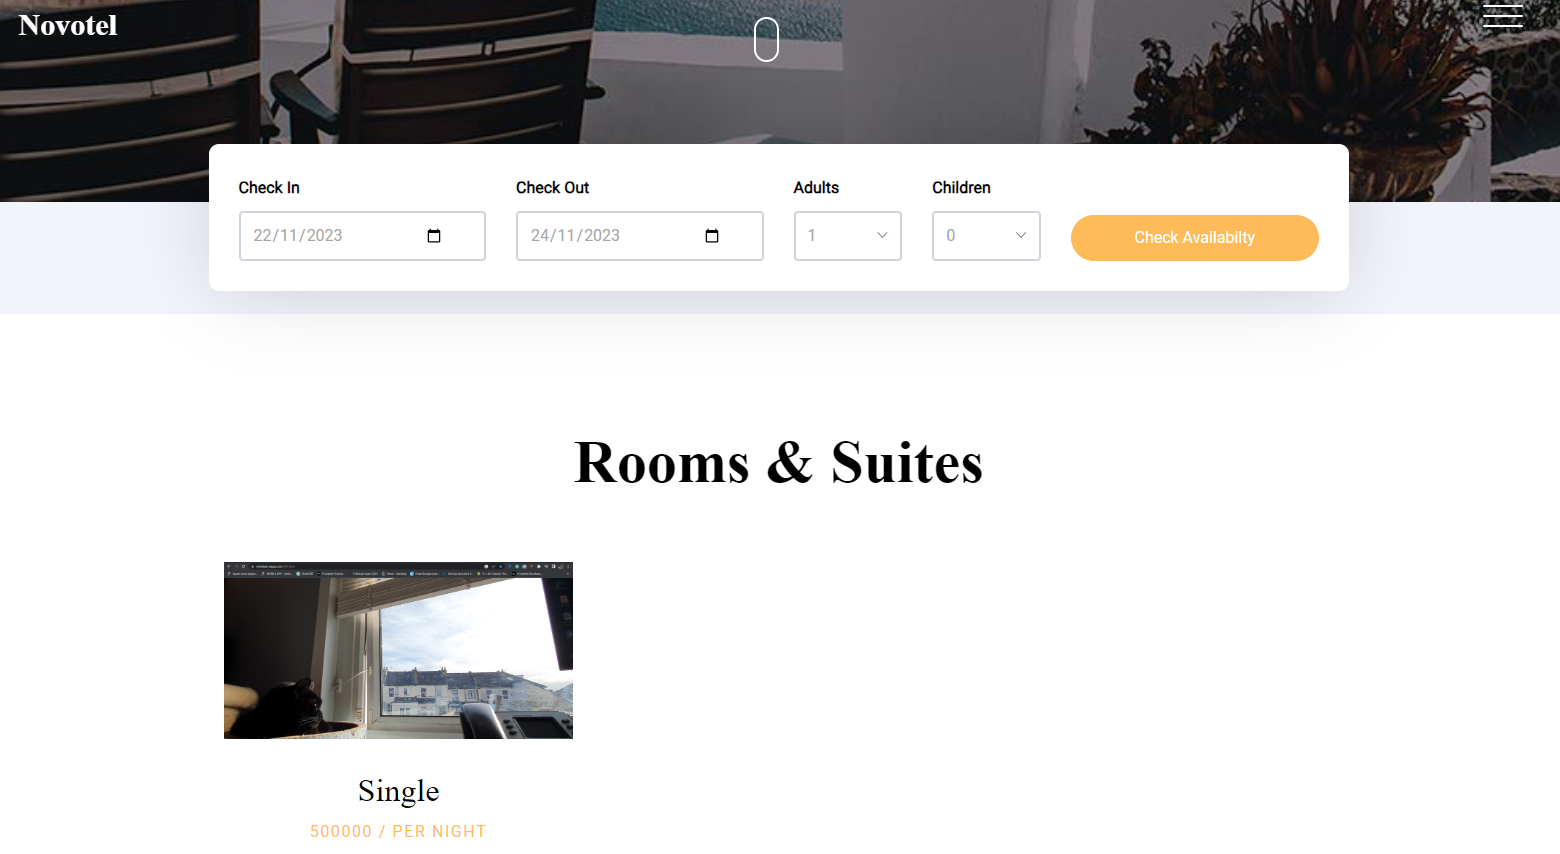
\includegraphics[width=1\linewidth]{img/checkavai.png}
            \label{fig:Checkavairoom}
        \end{figure}
        \item If the hotel has no available rooms, it will return no available rooms.
        \begin{figure}[H]
            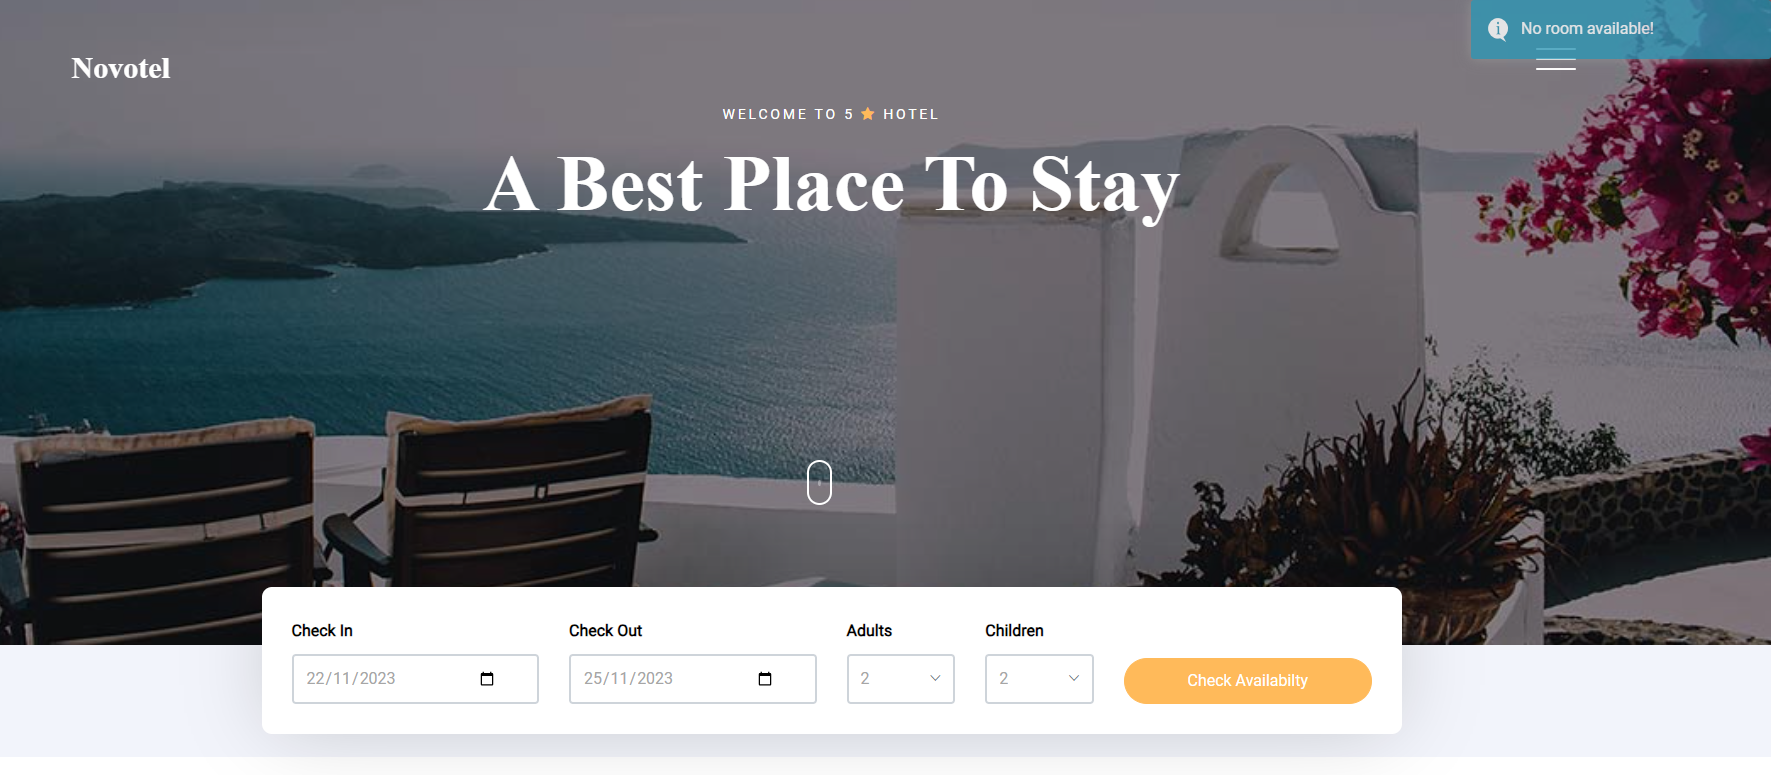
\includegraphics[width=1\linewidth]{img/noroomavai.png}
            \label{fig:NoRoomavai}
        \end{figure}
        \item If the Actor does not completely fill in the fields, an error message will be reported.
        \begin{figure}[H]
            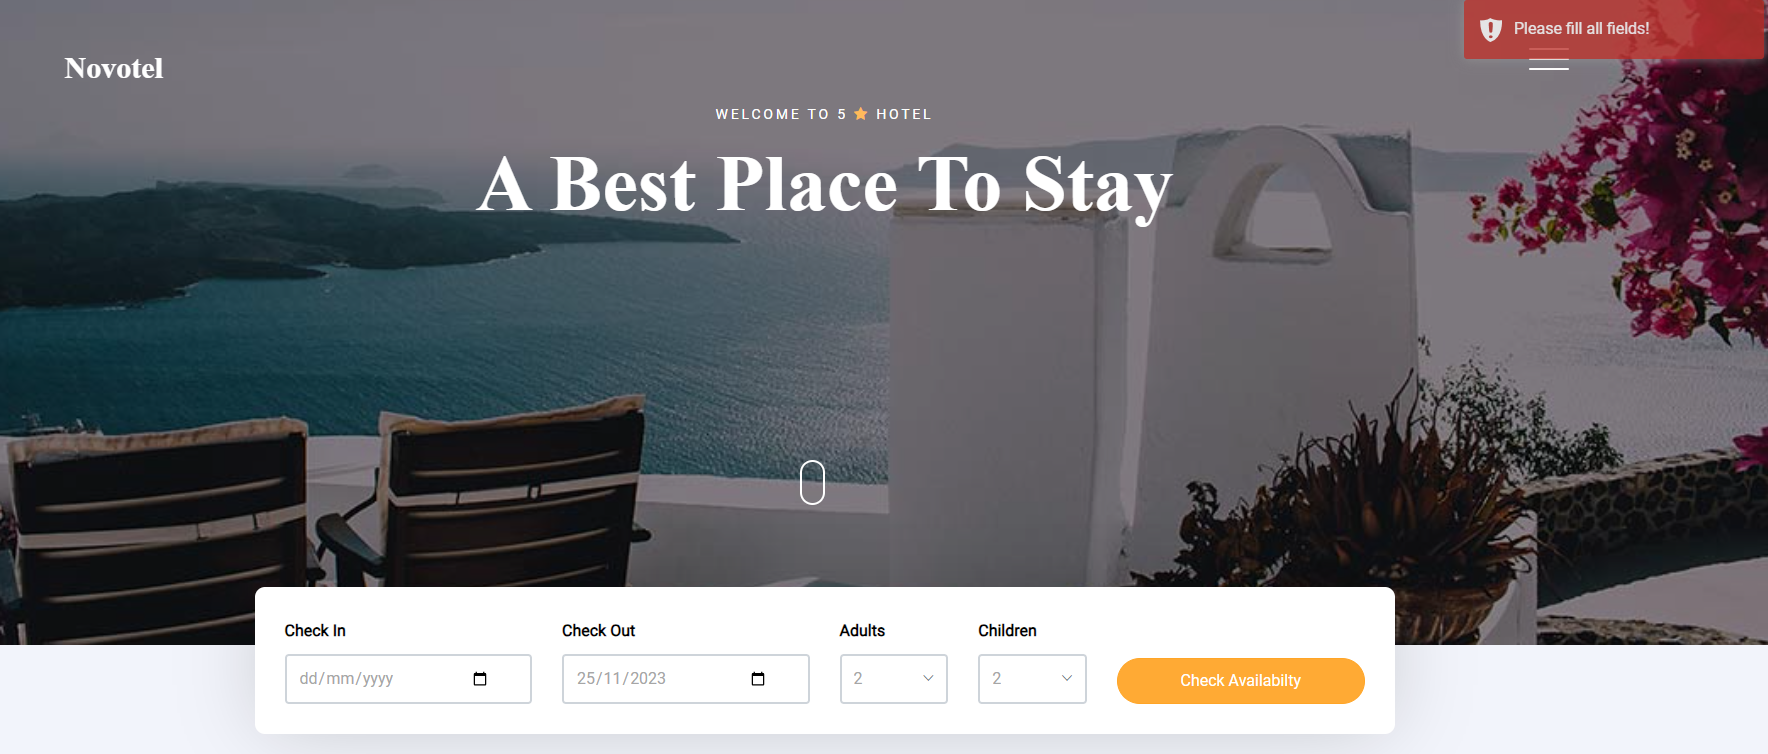
\includegraphics[width=1\linewidth]{img/dontfillalll.png}
            \label{fig:dontfillall}
        \end{figure}
    \end{itemize}
    \subsection{Booking}
    \begin{itemize}
        \item Receptionist and manager fill in all fields for the room search and select available rooms.
        \begin{figure}[H]
            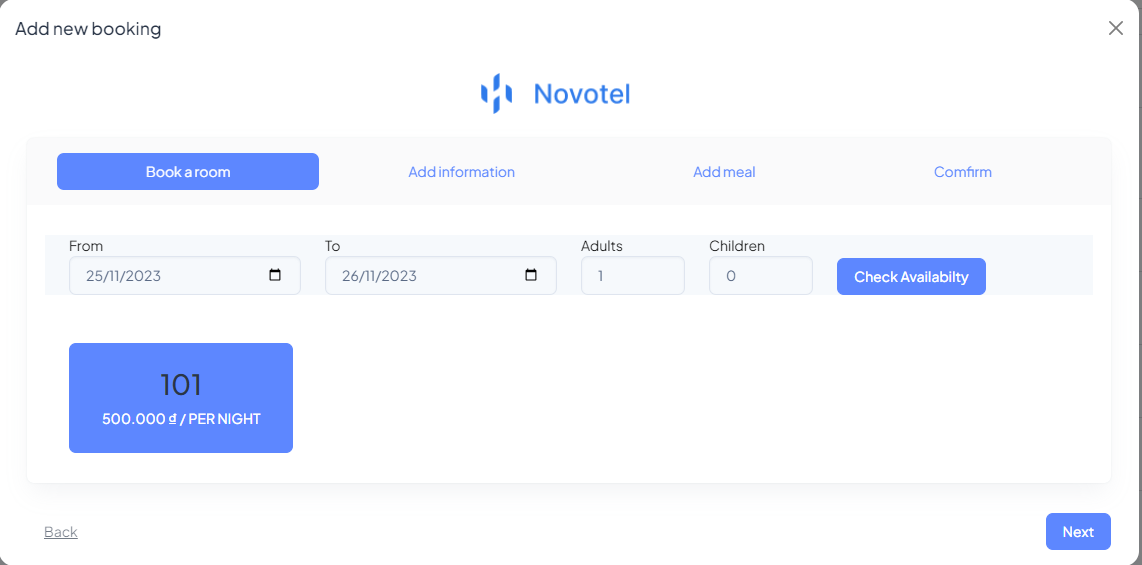
\includegraphics[width=1\linewidth]{img/bookroom.png}
            \label{fig:bookroom}
        \end{figure}
        \item Continue filling in tenant information. If you want to use the airport shuttle service, please select the type of vehicle you want and fill in all relevant fields. If guests have special service requests, they will be recorded.
        \begin{figure}[H]
            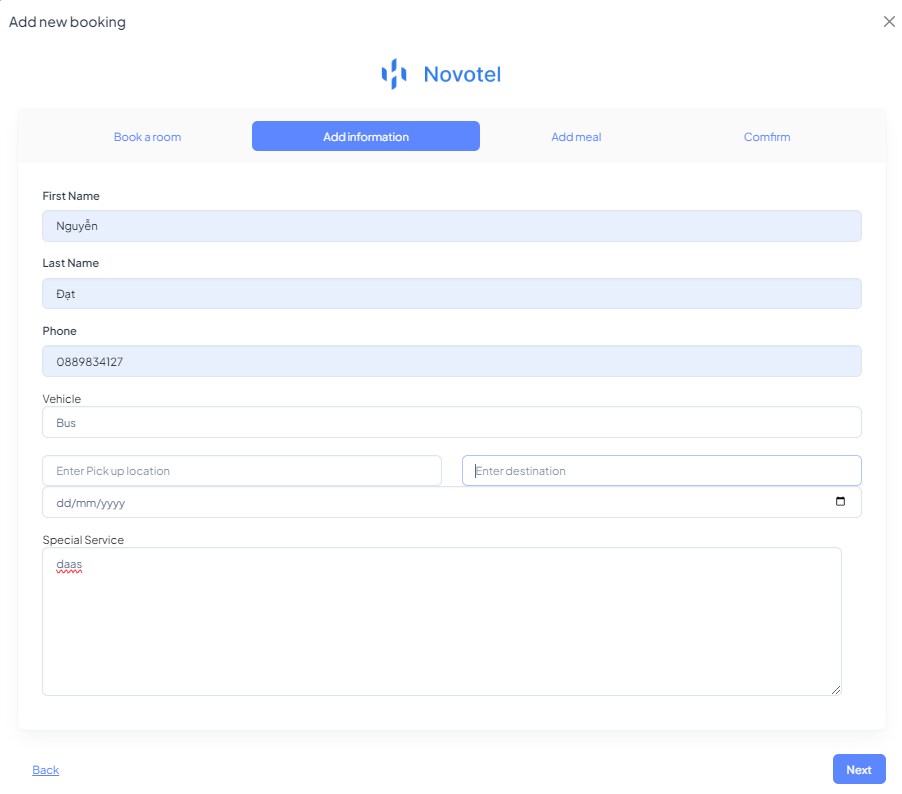
\includegraphics[width=1\linewidth]{img/addinfor.png}
            \label{fig:addinfor_room}
        \end{figure}
        \item If the guest needs to eat food, they will choose the food according to the guest's request.
        \begin{figure}[H]
            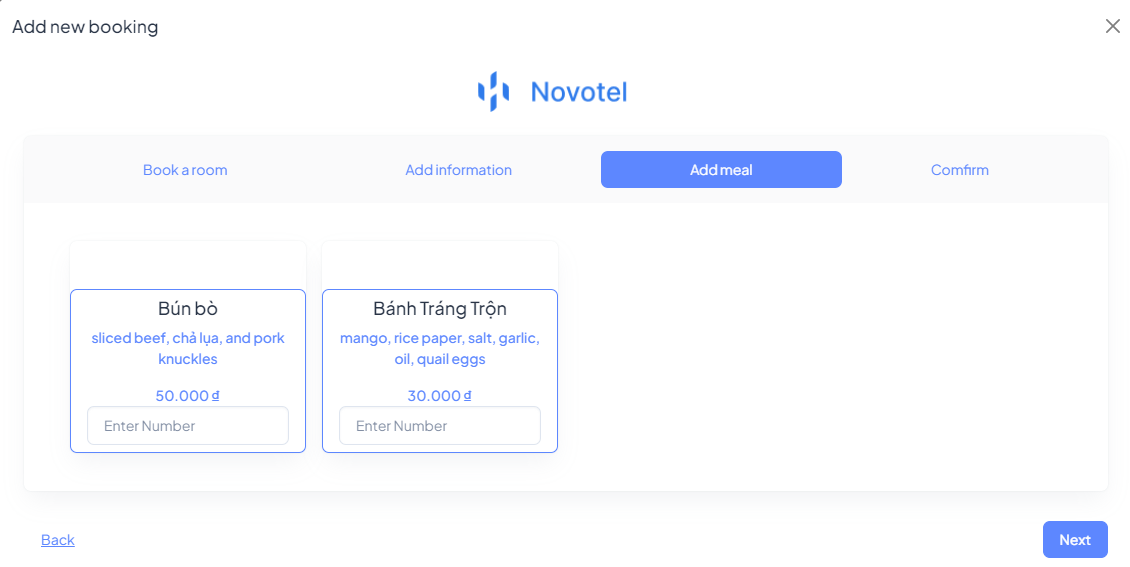
\includegraphics[width=1\linewidth]{img/bookmeal.png}
            \label{fig:bookmealroom}
        \end{figure}
        \item Finally, the actor will confirm the booking and other services.
    \end{itemize}
    \subsection{Update Booking}
    \begin{itemize}
        \item Receptionist and manager edit information about services, status,guest information, vehicles, or notes.
        \begin{figure}[H]
            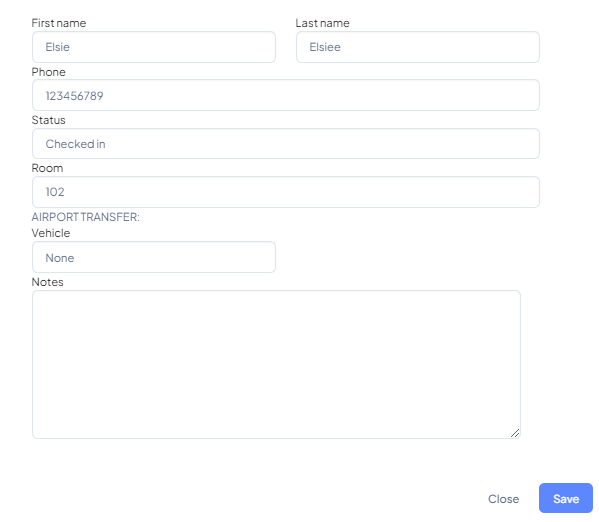
\includegraphics[width=1\linewidth]{img/editbookroom.png}
            \label{fig:editbookroom}
        \end{figure}
    \end{itemize}
    \subsection{Cancel Booking}
    \begin{itemize}
        \item Receptionist and manager change the room's status to canceled and will cancel the booking from the guest.
        \begin{figure}[H]
            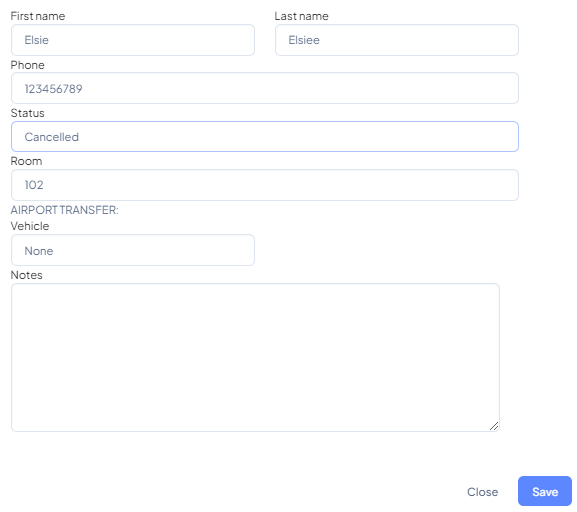
\includegraphics[width=1\linewidth]{img/cancelbook.png}
            \label{fig:cancelbook}
        \end{figure}
    \end{itemize}

    \subsection{View room information}
    \begin{itemize}
        \item Guest views detail information about the room (images, price) on the home page.
        \begin{figure}[H]
            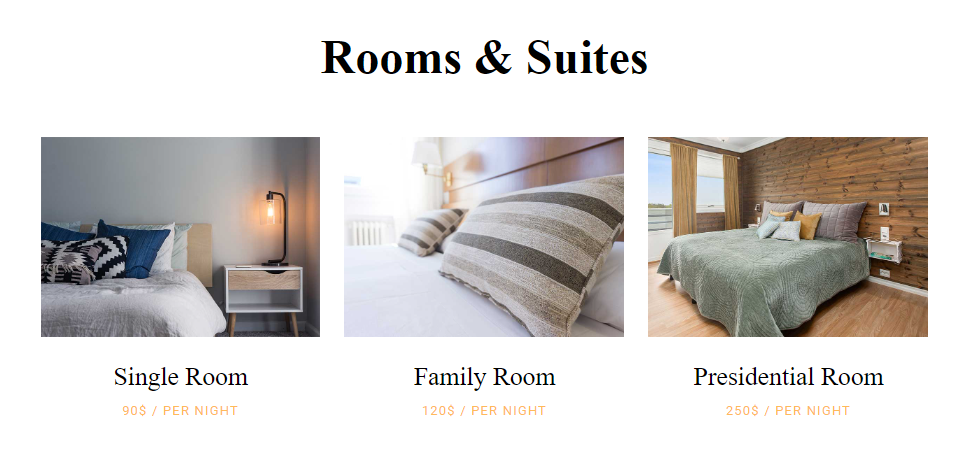
\includegraphics[width=1\linewidth]{img/viewroomin4.png}
            \label{fig:viewroominfor}
        \end{figure}
        \item Manager and receptionist view detail information about the room (images, price, facilities, status,etc).
        \begin{figure}[H]
            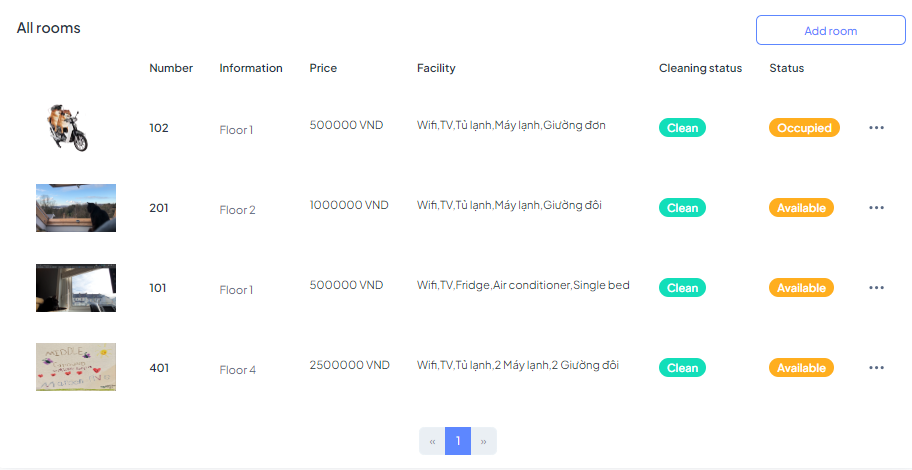
\includegraphics[width=1\linewidth]{img/viewroom_admin.png}
            \label{fig:viewroominfor_admin}
        \end{figure}
    \end{itemize}
    \subsection{Book meal}
    \begin{itemize}
        \item If the guest needs to eat food, manager or receptionist will choose the food according to the guest's request.
        \begin{figure}[H]
            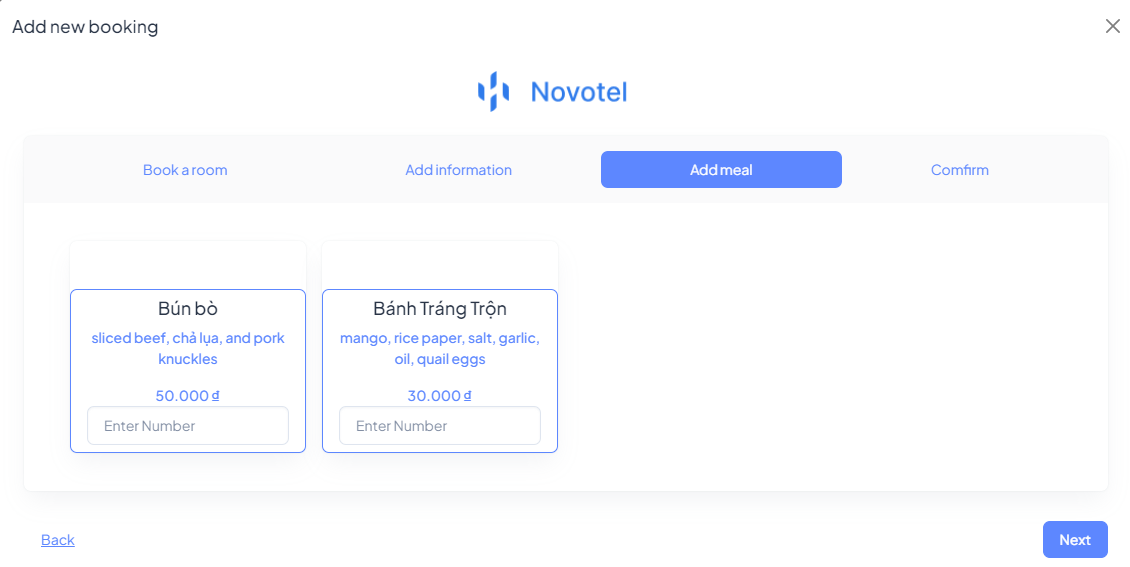
\includegraphics[width=1\linewidth]{img/bookmeal.png}
            \label{fig:bookmeal}
        \end{figure}
    \end{itemize}
    \subsection{Book airport transfer service}
    \begin{itemize}
        \item  If guest want to use the airport shuttle service, manager or receptionist select the type of vehicle guest want and fill in all relevant fields such as pick up location, pick up date and destination.
        \begin{figure}[H]
            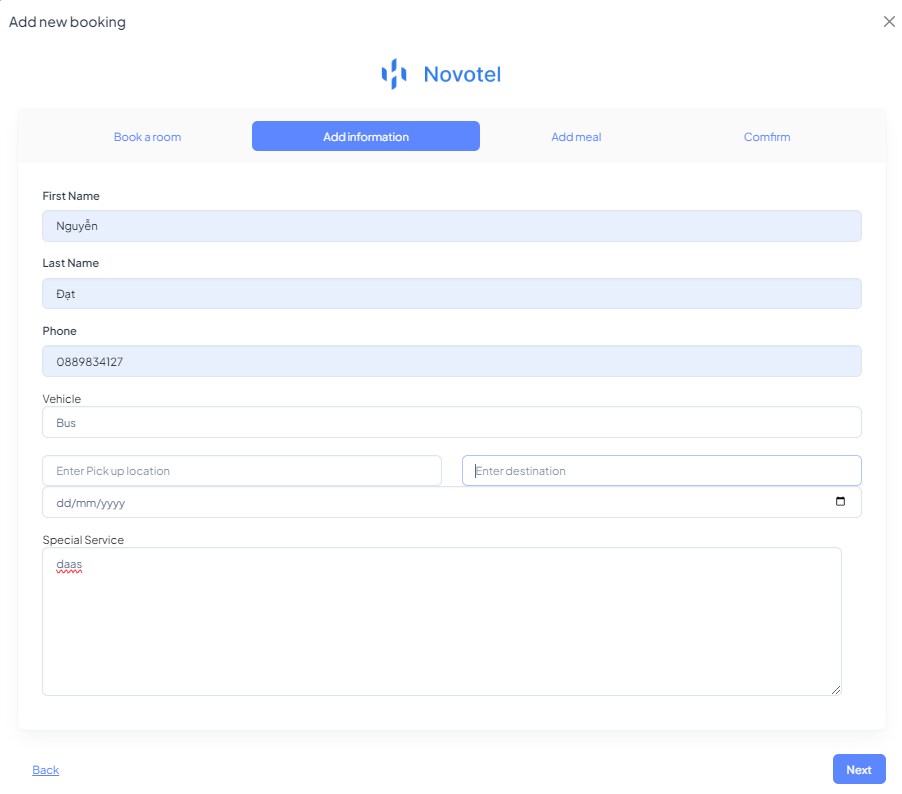
\includegraphics[width=1\linewidth]{img/addinfor.png}
            \label{fig:bookvehicle}
        \end{figure}
    \end{itemize}
    \subsection{Check-in}
    \begin{itemize}
        \item Receptionist and manager confirm that the room has been booked by the guest (guest check-in time). 
        \begin{figure}[H]
            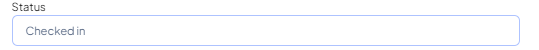
\includegraphics[width=1\linewidth]{img/checkin.png}
            \label{fig:checkin}
        \end{figure}
    \end{itemize}
    \subsection{Check-out}
    \begin{itemize}
        \item Receptionist and manager change the room's status to check-out and receptionist or manager confirm that the guest has left the room (guest check-out time)
        \begin{figure}[H]
            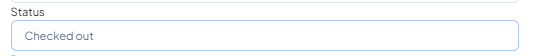
\includegraphics[width=1\linewidth]{img/checkout.png}
            \label{fig:checkout}
        \end{figure}
    \end{itemize}
    \subsection{Send feedback}
    \begin{itemize}
        \item Guest send reviews about hotel quality, service, and staff attitude to the hotel.
        \item Receptionist send feedback on the status of the facility, guest issues, and others.
        \begin{figure}[H]
            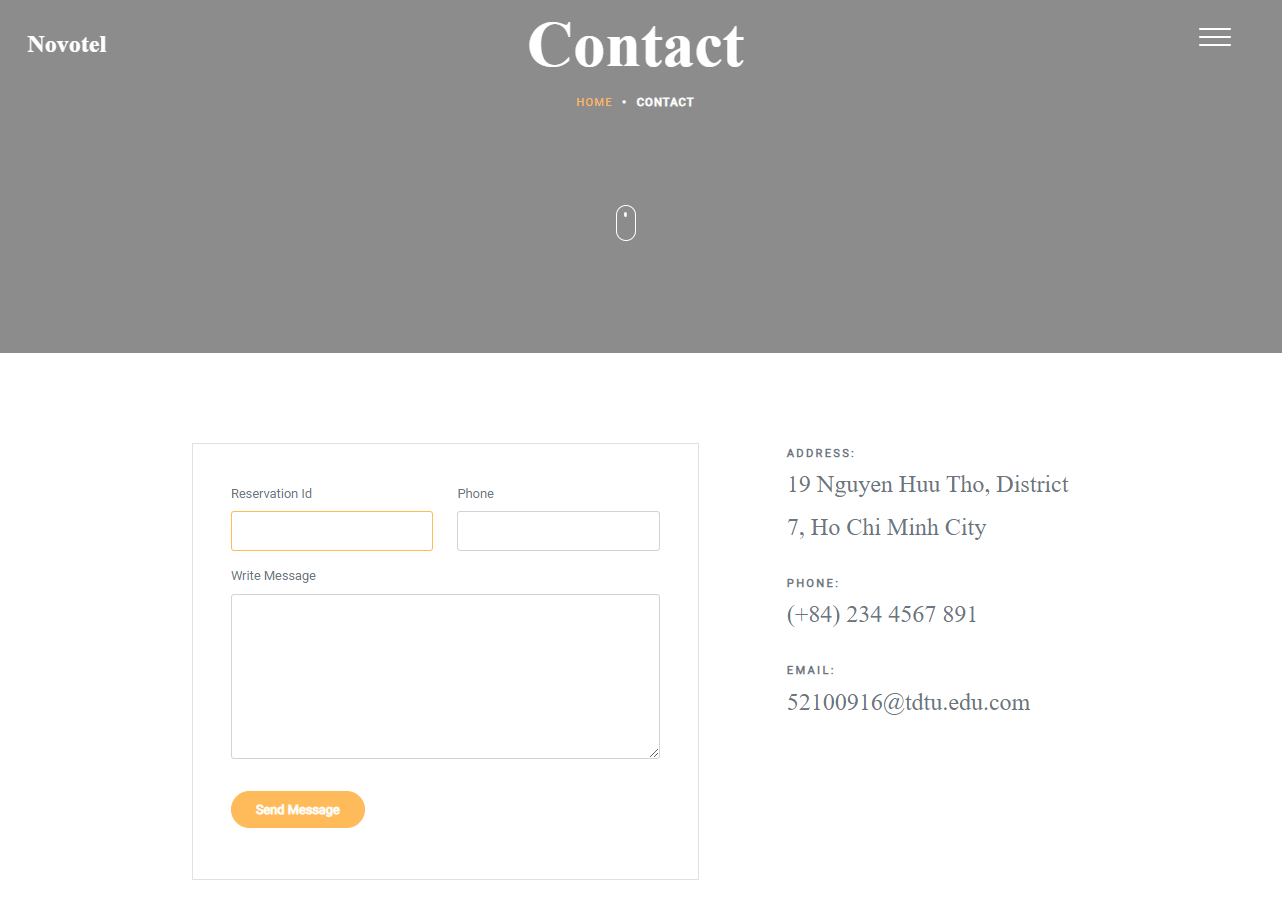
\includegraphics[width=1\linewidth]{img/sendfeed.png}
            \label{fig:sendfeedback}
        \end{figure}
    \end{itemize}
    \subsection{Find Invoice}
    \begin{itemize}
        \item Manager and accountant search for invoices that have been created in "Invoice" on the toolbar to see detailed information about these invoices.
        \begin{figure}[H]
            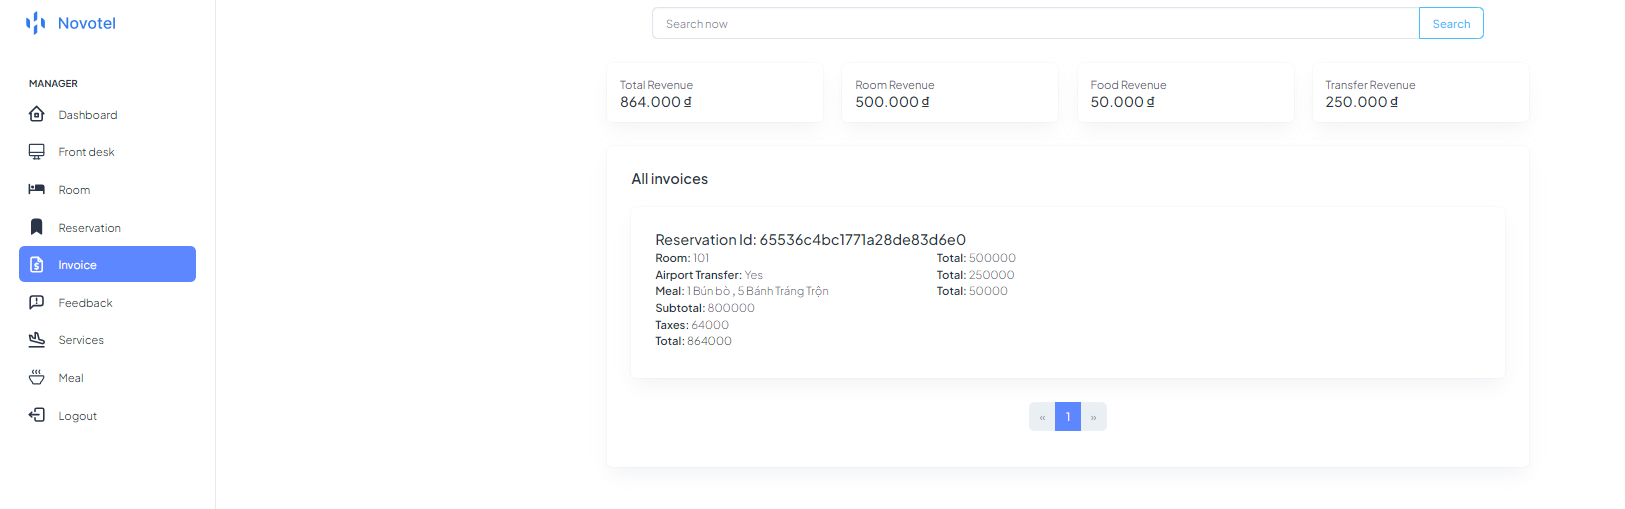
\includegraphics[width=1\linewidth]{img/findinvoice.png}
            \label{fig:findinvoice}
        \end{figure}
    \end{itemize}
    \subsection{View invoice history}
    \begin{itemize}
        \item Manager and accountant review invoice history to perform hotel revenue statistics in "Invoice" on the toolbar.
        \begin{figure}[H]
            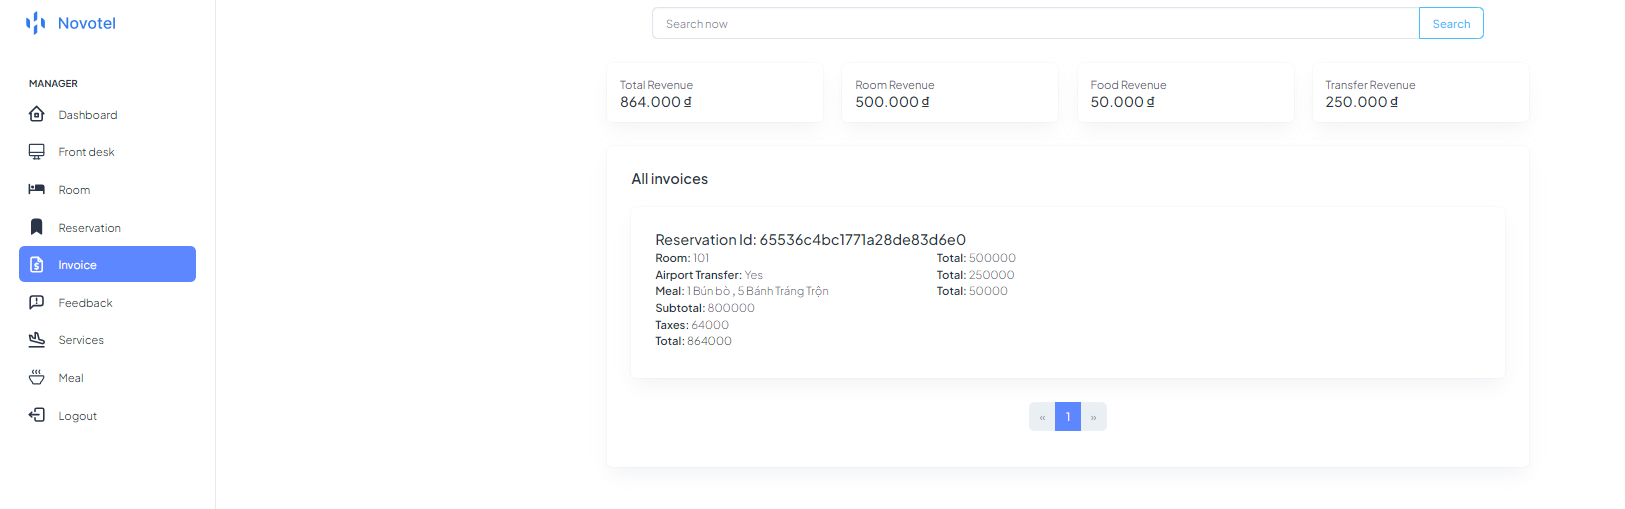
\includegraphics[width=1\linewidth]{img/findinvoice.png}
            \label{fig:viewinvoice}
        \end{figure}
    \end{itemize}
    \subsection{Manage room}
    \begin{itemize}
        \item Manager clicks on the ”Room” on the toolbar.
        \item The manager chooses the function he wants to perform:
        \begin{itemize}
            \item If the manager chooses to add or edit room information. After entering or adjusting all information about the room that needs to be adjusted (or added), the manager clicks on "Add" or "Save", and the room information in the hotel is automatically added to the database table.
            \begin{figure}[H]
                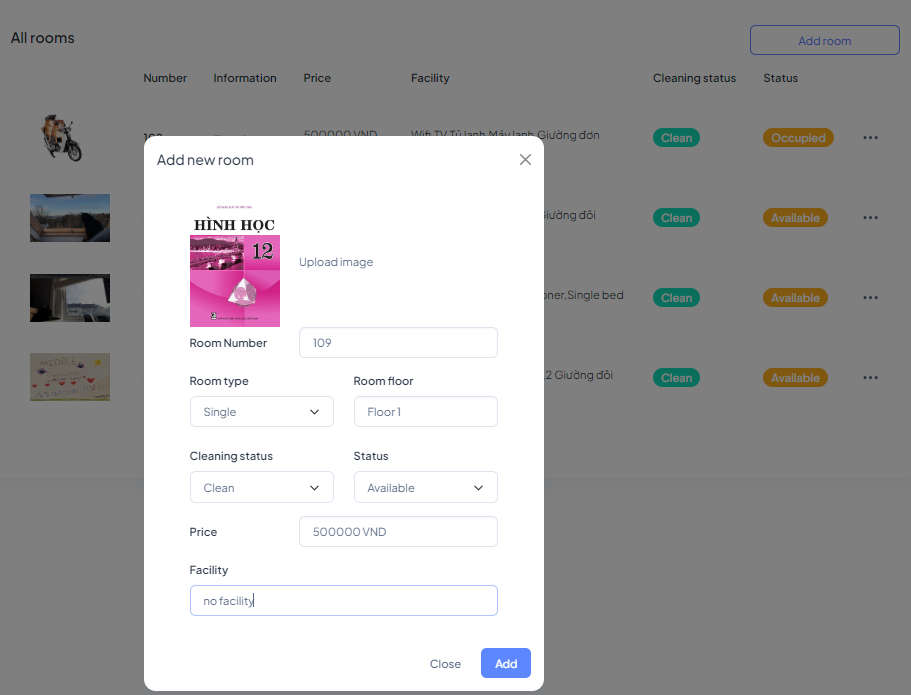
\includegraphics[width=1\linewidth]{img/addroom.png}
                \label{fig:addroom}
            \end{figure}
            \begin{figure}[H]
                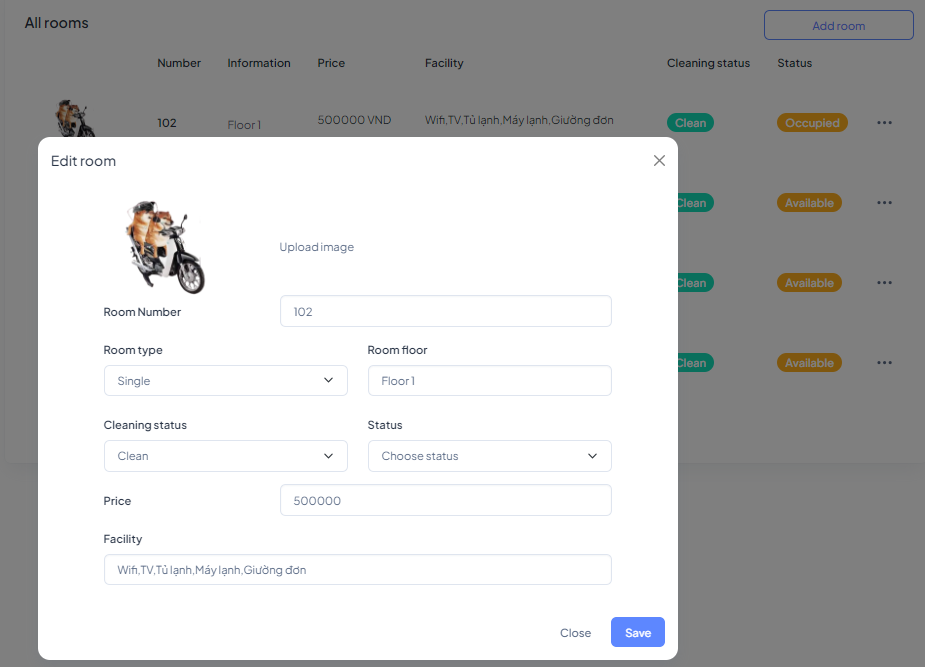
\includegraphics[width=1\linewidth]{img/editroom.png}
                \label{fig:editroom}
            \end{figure}
            \item If the manager chooses to delete, the system requires the manager to enter the exact room code to be deleted and then confirm that information about that room will be deleted from the system's database table.
            \begin{figure}[H]
                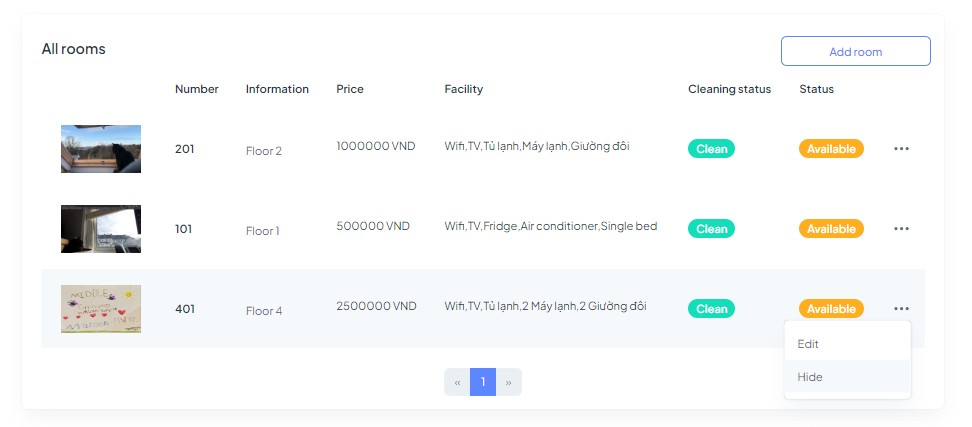
\includegraphics[width=1\linewidth]{img/deleteroom.png}
                \label{fig:deleteroom}
            \end{figure}
        \end{itemize}
    \end{itemize}
    \subsection{Manage Reservation}
    \begin{itemize}
        \item Manager clicks on the ”Room” on the toolbar.
        \item The manager chooses the function he wants to perform:
        \item If the manager chooses to edit reservation information. After adjusting information about the reservation that needs to be adjusted, the manager clicks "Save", and the reservation information in the hotel is automatically added to the database table.
        \begin{figure}[H]
            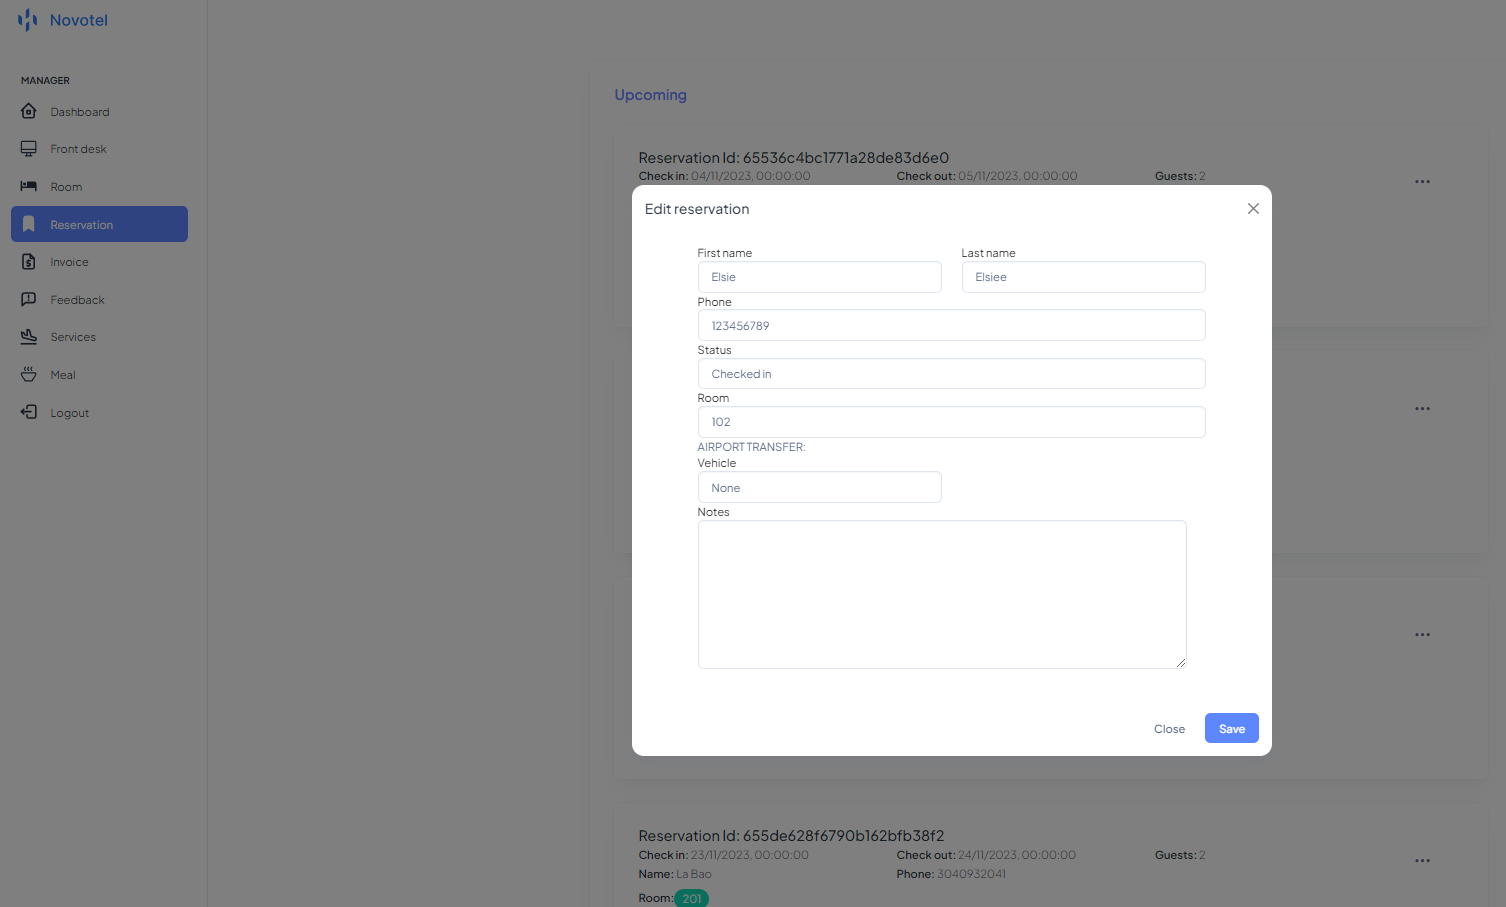
\includegraphics[width=1\linewidth]{img/editreservation.png}
            \label{fig:editreservation}
        \end{figure}
        \item If the manager chooses to add meals. They will select the meal and quantity then press "Save". This is done when guests need food.
        \begin{figure}[H]
            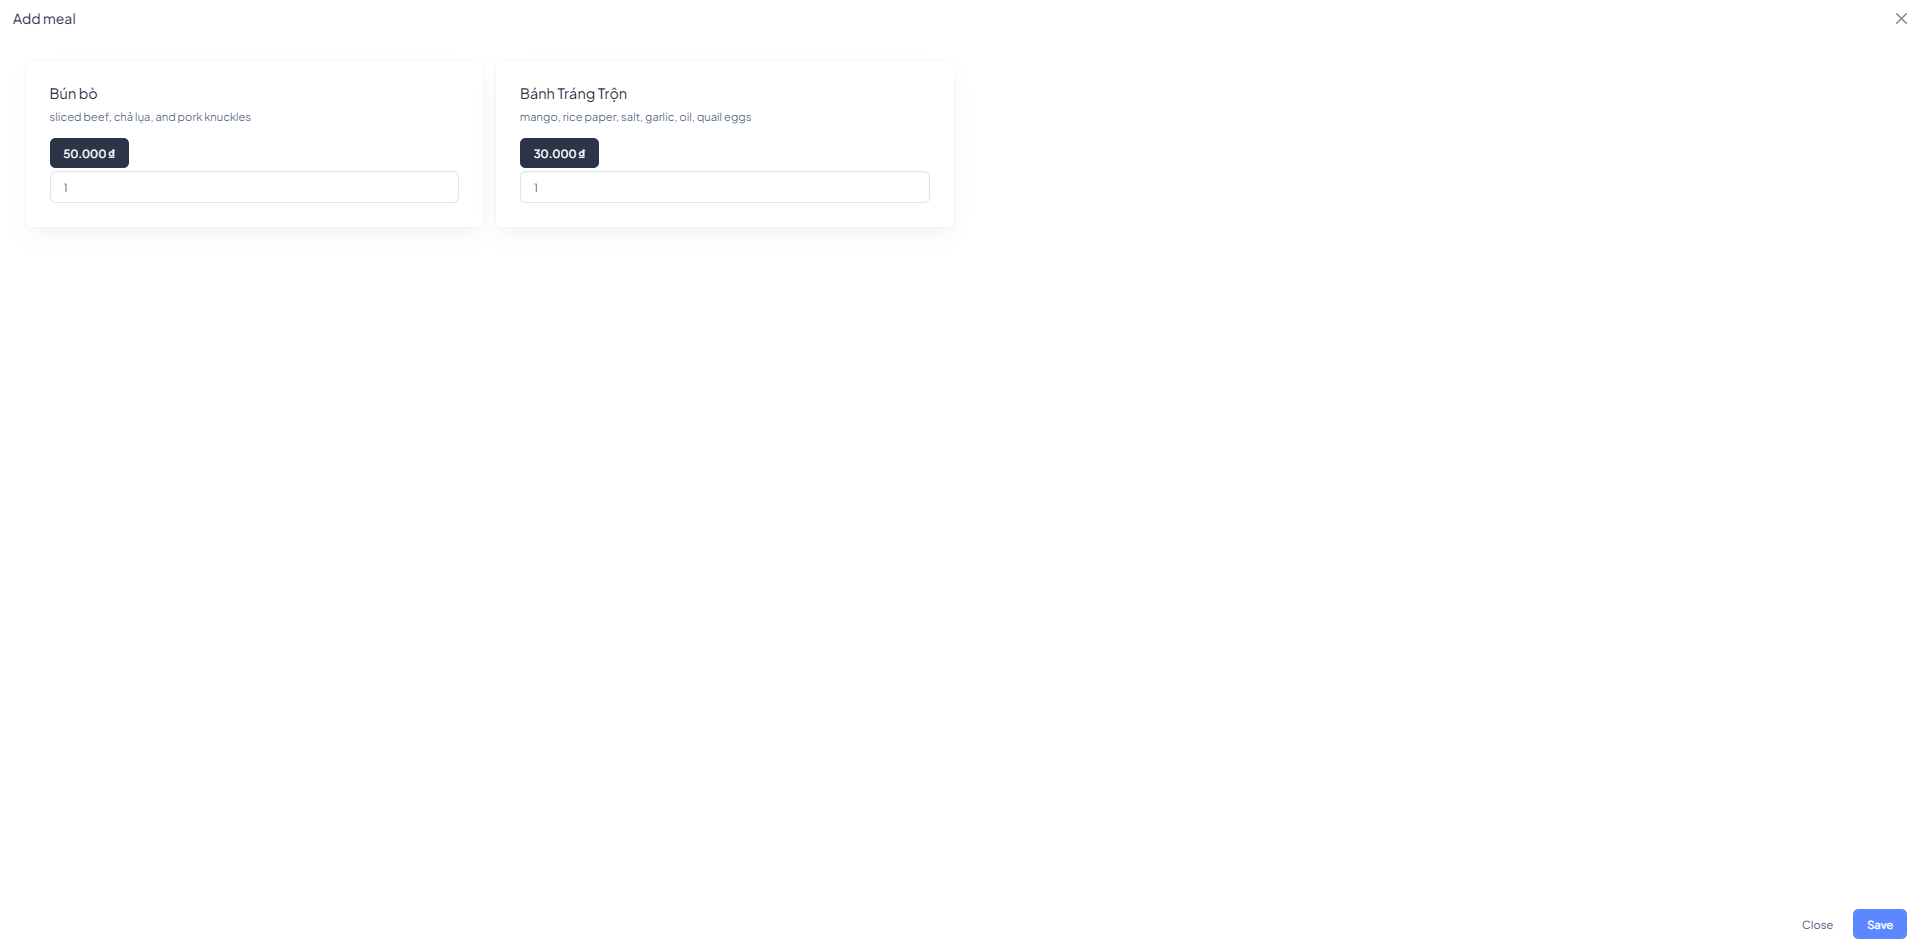
\includegraphics[width=1\linewidth]{img/Addmeal_reservation.png}
            \label{fig:addmeal_reservation}
        \end{figure}
    \end{itemize}
    \subsection{Manage menu item}
    \begin{itemize}
        \item Manager clicks on ”Meal” on the toolbar.
        \item The manager chooses the function he wants to perform:
        \begin{itemize}
            \item If the manager chooses to add or edit meal information. After entering or adjusting all information about the meal that needs to be adjusted (or added), the manager clicks on "Add" or "Save", and the meal information in the hotel is automatically added to the database table.
            \begin{figure}[H]
                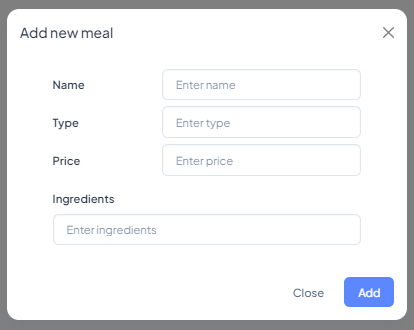
\includegraphics[width=1\linewidth]{img/addmeal_menu.png}
                \label{fig:addmeal_menu}
            \end{figure}
            \begin{figure}[H]
                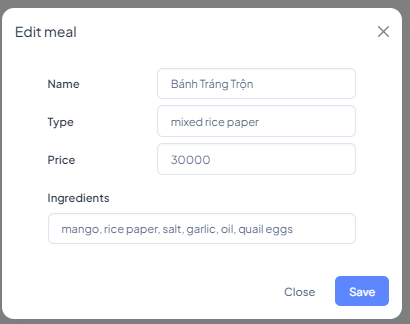
\includegraphics[width=1\linewidth]{img/editmeal.png}
                \label{fig:editmeal}
            \end{figure}
            \item If the manager chooses to delete, the system requires the manager to enter the exact meal code to be deleted and then confirm that information about that meal will be deleted from the system's database table.
            \begin{figure}[H]
                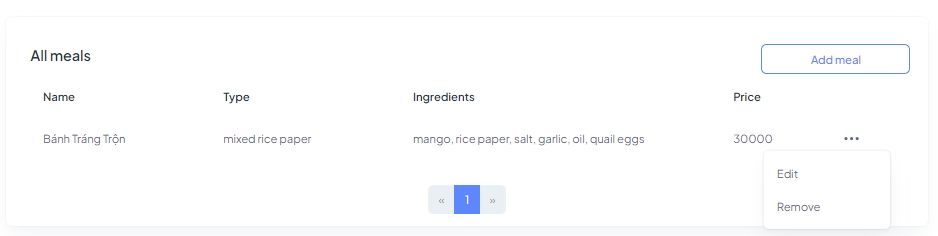
\includegraphics[width=1\linewidth]{img/deletemeal.png}
                \label{fig:deletemeal}
            \end{figure}
        \end{itemize}
    \end{itemize}
    \subsection{Review guest’s feedback}
    \begin{itemize}
        \item Manger click "Feedback" on the right toolbar of the website. The system will display a list of all the feedback that guests have sent to the hotel. Managers can choose to resolve feedback coming from guest.
        \begin{figure}[H]
                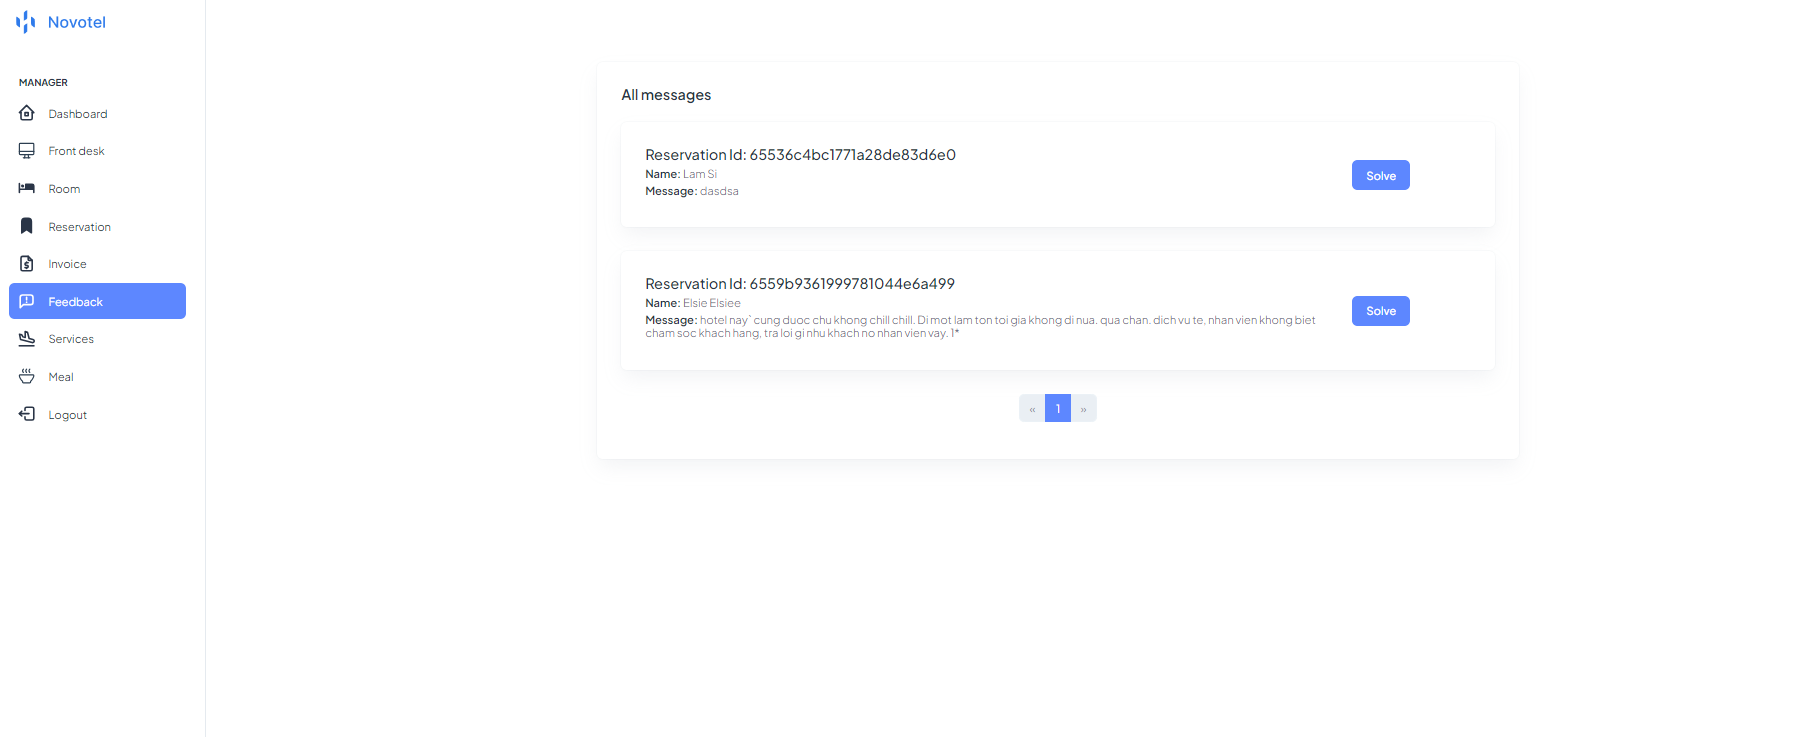
\includegraphics[width=1\linewidth]{img/rv_feedback.png}
                \label{fig:rvfeedback}
            \end{figure}
    \end{itemize}
    \subsection{View all airport transfer services}
    \begin{itemize}
        \item Manger click "Services" on the right toolbar of the website. The system will display a list of all guests who have used the hotel's airport transport service.
        \begin{figure}[H]
            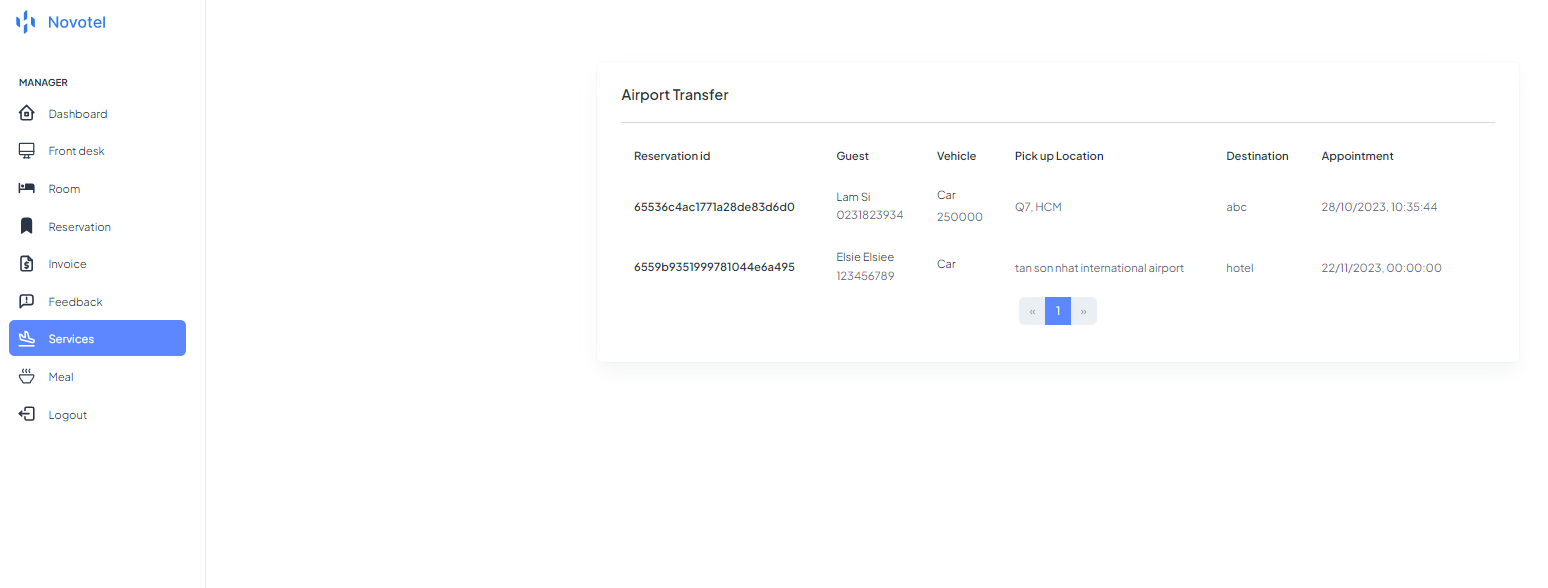
\includegraphics[width=1\linewidth]{img/transport.png}
            \label{fig:transport}
        \end{figure}
    \end{itemize}
    
    


